\documentclass[a4paper,10pt,twocolumn]{article}

\usepackage[utf8]{inputenc}
\usepackage[T1]{fontenc}
\usepackage[margin=2cm]{geometry}
\usepackage{amsmath,amssymb}
\usepackage{graphicx}
\usepackage{booktabs}
\usepackage{caption}
\usepackage{subcaption}
\usepackage{hyperref}
\usepackage{xcolor}
\usepackage{enumitem}

\title{
  \textbf{EA-VTON: Ethnicity-Aware Virtual Try-On} \\
  \textbf{Prototype Status and Current Results}
}

\author{
  Nguyen Thi Anh Tho \and Le Thanh Danh \\
  International University, VNU-HCMC
}

\date{April 2, 2026}

\begin{document}
\maketitle

\begin{abstract}
Virtual try-on systems have improved rapidly, but most current pipelines still assume body priors and size logic derived from Western-centric datasets. This creates a mismatch for Vietnamese users in both garment visualization and size recommendation. This paper summarizes the current status of \textbf{EA-VTON}, an ethnicity-aware virtual try-on prototype targeted at Vietnamese body characteristics. The current implementation includes a web interface, a FastAPI backend, a FASHN VTON v1.5 test pipeline, post-hoc garment-only compositing, and a Vietnamese-aware size recommendation comparison module. On an Apple M2 CPU, the prototype supports a fast 3-step preview path and a 10/20/30-step benchmark path. Current results indicate that 20 inference steps provide the best quality-cost tradeoff among the tested settings. The full population-specific body modeling stage, including VN-SMPL and synthetic Vietnamese body generation, remains future work, but the present prototype already provides a working system for demonstrating the EA-VTON research direction.
\end{abstract}

\section{Introduction}
\label{sec:intro}

Image-based virtual try-on (VTON) has progressed from warping-based methods such as VITON~\cite{han2018viton} and CP-VTON~\cite{wang2018cpvton} to diffusion-based methods such as IDM-VTON~\cite{choi2023idmvton} and CatVTON~\cite{choi2024catvton}. These systems improve realism, but they generally remain population-agnostic: body shape priors, size charts, and training distributions are dominated by Western or global-average data.

For Vietnamese users, this creates two practical problems. First, the displayed garment fit may not reflect local body proportions accurately. Second, size recommendation logic trained on Western-centric data tends to oversize relative to Vietnamese body statistics. The long-term goal of EA-VTON is to address both issues through population-aware body modeling and size recommendation.

This paper focuses on the \textit{current prototype}. The present repository does not yet implement VN-SMPL end-to-end. Instead, it provides a complete system prototype that already supports:
\begin{itemize}[leftmargin=*, itemsep=2pt]
  \item a working frontend for upload, garment selection, and result display,
  \item a backend try-on pipeline using FASHN VTON v1.5,
  \item garment-only postprocessing to preserve the wearer and background,
  \item and a Vietnamese-aware size comparison module.
\end{itemize}

\section{Current Prototype}
\label{sec:prototype}

\subsection{System Overview}

The current EA-VTON prototype consists of a Next.js frontend and a FastAPI backend. The frontend provides pages for landing, catalog browsing, product details, try-on, and result display. The backend exposes routes for photo upload, try-on jobs, garments, and size recommendation comparison.

The implemented runtime flow is:
\begin{enumerate}[leftmargin=*, itemsep=2pt]
  \item upload or capture a user photo,
  \item select a garment from the demo catalog,
  \item run try-on inference,
  \item apply garment-only postprocessing,
  \item return the final image and size recommendation.
\end{enumerate}

\begin{figure}[t]
  \centering
  \includegraphics[width=0.9\linewidth]{../../fitview-homepage.png}
  \caption{Current web interface used to demonstrate the EA-VTON prototype.}
  \label{fig:homepage}
\end{figure}

\subsection{Try-On Pipeline}

The current inference backend uses \texttt{fashn-ai/fashn-vton-1.5}. In contrast to pipelines that require a garment mask at inference time, the current prototype uses the model in a mask-free way for generation and then detects the garment region afterward.

The backend stages are:
\begin{enumerate}[leftmargin=*, itemsep=2pt]
  \item person and garment preprocessing,
  \item VTON inference,
  \item garment-region detection,
  \item garment-only enhancement and compositing,
  \item quality reporting.
\end{enumerate}

\subsection{Garment-Only Postprocessing}

The key implementation detail in the current prototype is that enhancement is restricted to the garment region. A garment mask is detected from the difference between the original image and the generated try-on result. Postprocessing is then applied only inside that mask. This reduces visible artifacts on the face, skin, hair, and background.

The final composition is:
\begin{equation}
I_{\text{final}} = I_{\text{orig}} \cdot (1 - M) + I_{\text{enhanced}} \cdot M
\end{equation}
where $M$ is the garment mask, $I_{\text{orig}}$ is the original user image, and $I_{\text{enhanced}}$ is the garment-enhanced try-on result.

\begin{figure}[t]
  \centering
  \begin{subfigure}[t]{0.31\linewidth}
    \centering
    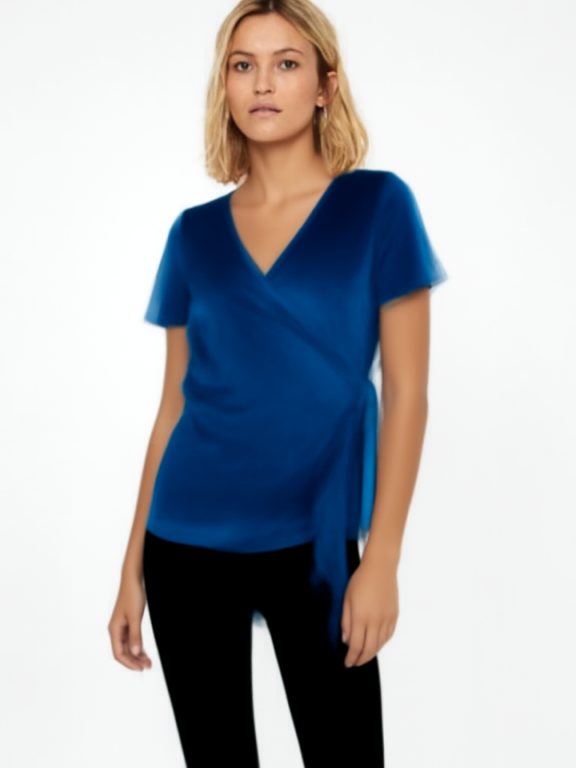
\includegraphics[width=\linewidth]{../../backend/test_results/output_raw.png}
    \caption{Raw preview}
  \end{subfigure}
  \hfill
  \begin{subfigure}[t]{0.31\linewidth}
    \centering
    
\includegraphics[width=\linewidth]{../../backend/test_results/garment_mask.png}
    \caption{Garment mask}
  \end{subfigure}
  \hfill
  \begin{subfigure}[t]{0.31\linewidth}
    \centering
    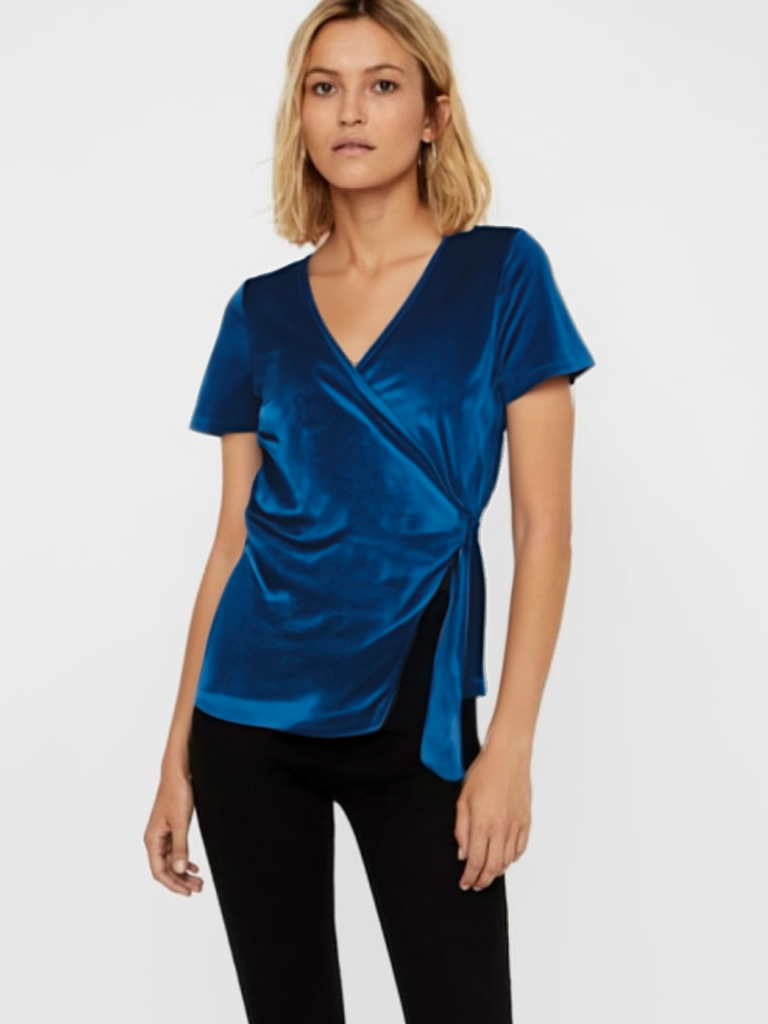
\includegraphics[width=\linewidth]{../../backend/test_results/output_final.png}
    \caption{Final result}
  \end{subfigure}
  \caption{Current garment-only postprocessing path. The mask is detected after inference and used to preserve non-garment regions.}
  \label{fig:garment_composite}
\end{figure}

\subsection{Vietnamese-Aware Size Comparison}

The current codebase also includes a population-aware size comparison module. At present, the implemented EA logic is a body-measurement estimation layer rather than a full body-model calibration stage. The system compares a universal chest estimate against a Vietnamese-adjusted estimate:
\begin{align}
\hat{c}_{\text{universal}} &= 0.52 \cdot h + 0.18 \cdot w \\
\hat{c}_{\text{VN}} &= 0.485 \cdot h + 0.22 \cdot w - 2.5
\end{align}
where $h$ is height in centimeters and $w$ is weight in kilograms. This comparison supports the main research claim that population-specific priors matter even before full VN-SMPL integration.

\section{Current Experimental Results}
\label{sec:results}

\subsection{Setup}

The current benchmark artifacts are stored in \texttt{backend/test\_results}. The reported setup is:
\begin{itemize}[leftmargin=*, itemsep=2pt]
  \item model: FASHN VTON v1.5,
  \item device: Apple M2 CPU,
  \item category: tops,
  \item seed: 42.
\end{itemize}

The repository currently supports two practical evaluation modes:
\begin{itemize}[leftmargin=*, itemsep=2pt]
  \item a fast \textbf{3-step preview} path for quick qualitative checks on Mac,
  \item a \textbf{10/20/30-step} benchmark path for quality-cost comparison.
\end{itemize}

\subsection{Step Comparison}

Table~\ref{tab:step_comparison} summarizes the available benchmark metrics. Among the tested settings, 20 steps provides the best balance of quality and runtime. The gain from 30 steps is relatively small compared to its additional CPU cost.

\begin{table}[t]
\centering
\caption{Current step comparison on Apple M2 CPU.}
\label{tab:step_comparison}
\small
\begin{tabular}{lcccc}
\toprule
\textbf{Steps} & \textbf{Inference} & \textbf{Face SSIM} & \textbf{Sharpness} & \textbf{Garment Detail} \\
\midrule
10 & 625.5s & 0.9344 & 41.2 & 55.2 \\
\textbf{20} & \textbf{953.0s} & \textbf{0.9345} & \textbf{44.1} & \textbf{57.6} \\
30 & 1511.5s & 0.9344 & 45.6 & 58.3 \\
\bottomrule
\end{tabular}
\end{table}

\begin{figure}[t]
  \centering
  \begin{subfigure}[t]{0.31\linewidth}
    \centering
    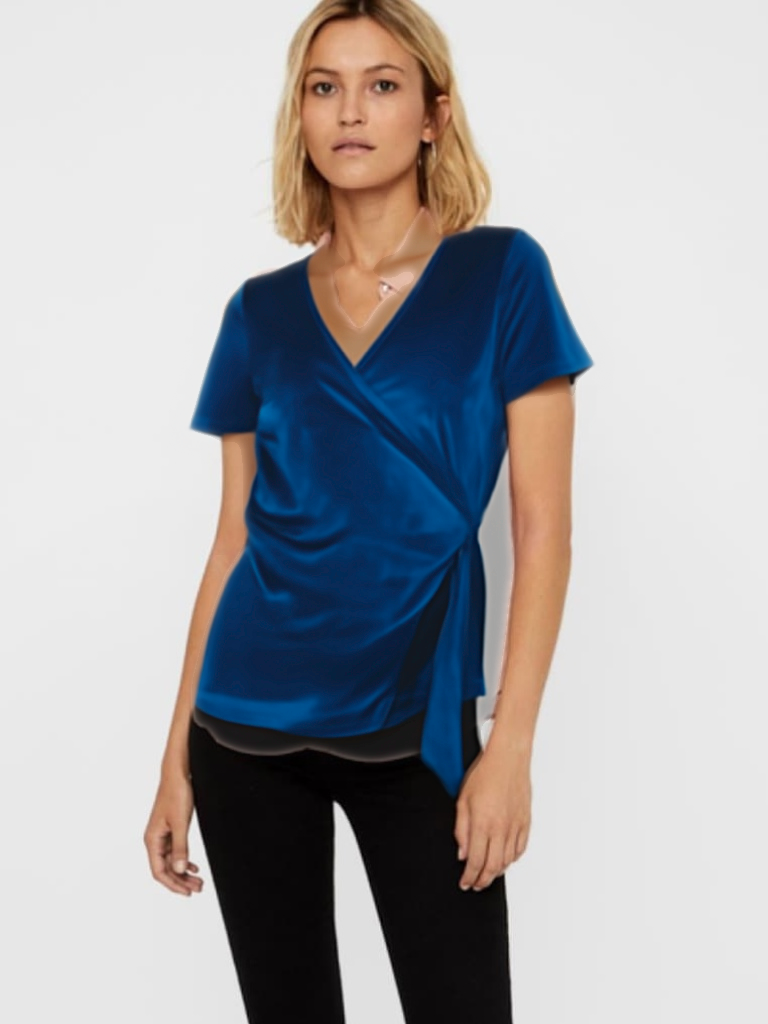
\includegraphics[width=\linewidth]{../../backend/test_results/step_comparison/final_10steps.png}
    \caption{10 steps}
  \end{subfigure}
  \hfill
  \begin{subfigure}[t]{0.31\linewidth}
    \centering
    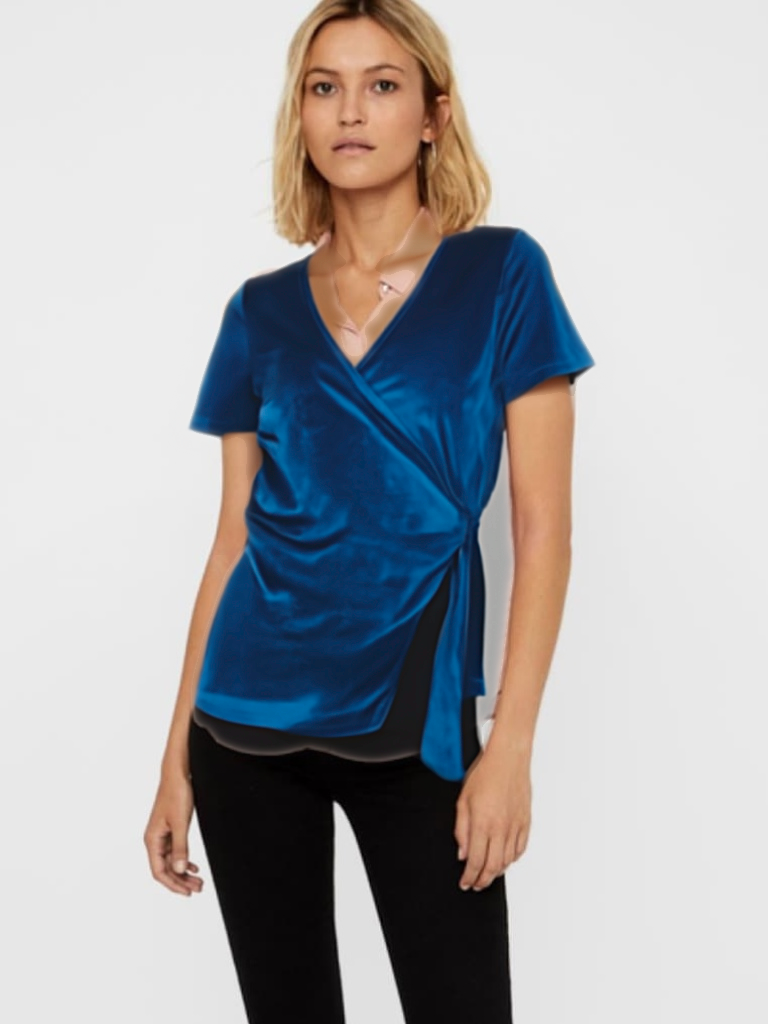
\includegraphics[width=\linewidth]{../../backend/test_results/step_comparison/final_20steps.png}
    \caption{20 steps}
  \end{subfigure}
  \hfill
  \begin{subfigure}[t]{0.31\linewidth}
    \centering
    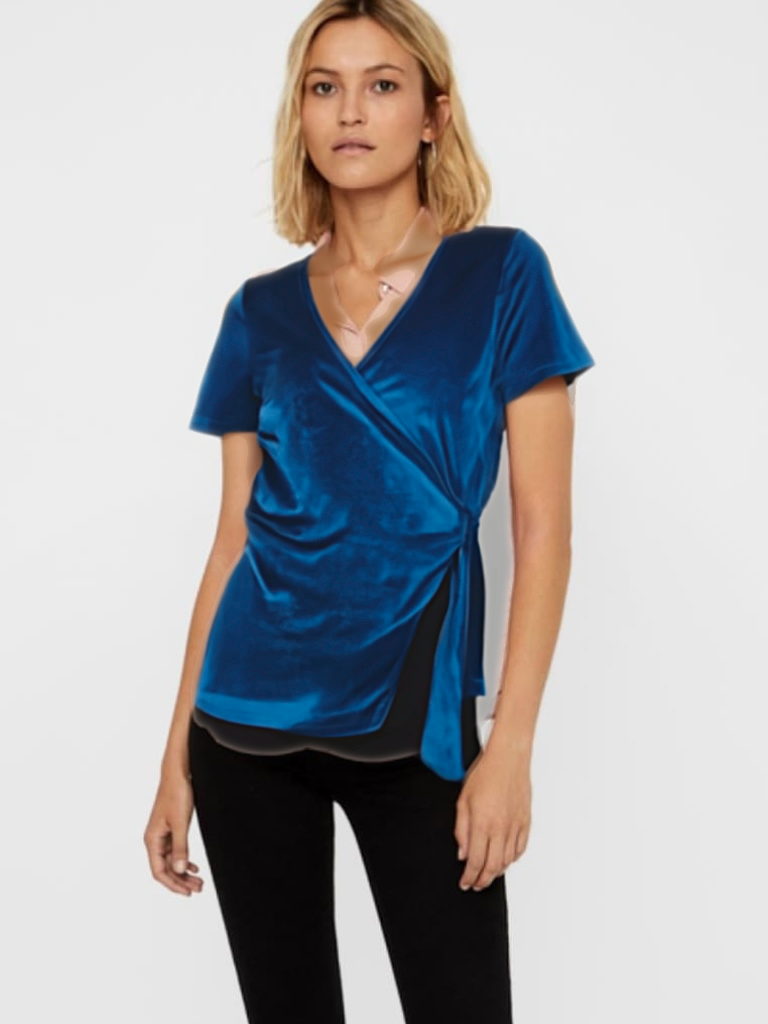
\includegraphics[width=\linewidth]{../../backend/test_results/step_comparison/final_30steps.png}
    \caption{30 steps}
  \end{subfigure}
  \caption{Current benchmark outputs. 20 steps offers a strong compromise between detail and runtime.}
  \label{fig:step_results}
\end{figure}

\subsection{Interpretation}

The current results support three practical conclusions:
\begin{itemize}[leftmargin=*, itemsep=2pt]
  \item The prototype can run on consumer Mac hardware for development and preview.
  \item Garment-only compositing is a meaningful improvement for preserving identity and background stability.
  \item The system is sufficiently mature for demonstrations, internal reporting, and further EA-specific integration work.
\end{itemize}

\section{Discussion and Next Steps}
\label{sec:discussion}

The current repository represents a \textit{prototype stage} rather than a completed research system. It already demonstrates the core user flow and provides quantitative signals for runtime-quality tradeoffs. However, several elements of the original EA-VTON vision remain future work.

\subsection{What Is Already Implemented}

\begin{itemize}[leftmargin=*, itemsep=2pt]
  \item web interface for the full user flow,
  \item backend orchestration for try-on jobs,
  \item FASHN VTON inference integration,
  \item garment-only postprocessing,
  \item Vietnamese-aware size comparison logic.
\end{itemize}

\subsection{What Remains Future Work}

\begin{itemize}[leftmargin=*, itemsep=2pt]
  \item VN-SMPL calibration from Vietnamese anthropometric data,
  \item synthetic Vietnamese body generation,
  \item tighter integration of population-aware body priors into try-on inference,
  \item broader quantitative evaluation on dedicated test sets.
\end{itemize}

In other words, the current system already supports the \textit{direction} of EA-VTON, but the full body-modeling contribution is still under construction.

\section{Conclusion}
\label{sec:conclusion}

This paper presented the current status of the EA-VTON prototype. The project has progressed from a concept into a working system with a usable frontend, a functioning try-on pipeline, garment-only postprocessing, and an initial Vietnamese-aware size comparison module. Current benchmark results on Apple M2 CPU show that the system supports both quick preview runs and deeper step-based quality comparisons, with 20 steps providing the best tested balance of quality and cost.

The next stage is to move from a prototype-level ethnicity-aware sizing layer toward full population-specific body modeling. That includes VN-SMPL, synthetic Vietnamese body generation, and broader evaluation. Even at its current stage, however, the prototype already serves as a concrete technical foundation for the EA-VTON research agenda.

\begin{thebibliography}{99}

\bibitem{han2018viton}
X. Han, Z. Wu, Z. Wu, R. Yu, and L.S. Davis, ``VITON: An image-based virtual try-on network,'' in \textit{CVPR}, 2018.

\bibitem{wang2018cpvton}
B. Wang, H. Zheng, X. Liang, Y. Chen, L. Lin, and M. Yang, ``Toward characteristic-preserving image-based virtual try-on network,'' in \textit{ECCV}, 2018.

\bibitem{choi2023idmvton}
S. Choi, S. Park, M. Lee, and J. Choo, ``Improving diffusion models for authentic virtual try-on in the wild,'' \textit{arXiv:2403.05139}, 2024.

\bibitem{choi2024catvton}
Z. Cheng, ``CatVTON: Concatenation is all you need for virtual try-on with diffusion models,'' in \textit{ICLR}, 2025.

\end{thebibliography}

\end{document}
